

\begin{minipage}[t]{.3\textwidth}
	\centering\raisebox{\dimexpr \topskip-\height}{%
	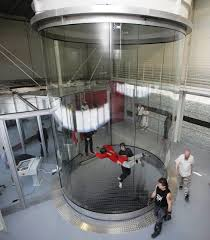
\includegraphics[scale=0.35]{tvert1.jpg}}
	\captionof{figure}{Tunel uso recreativo}
	\label{fig:tunelRec}
\end{minipage}	
\begin{minipage}[t]{.7\textwidth}

Un túnel de viento es una herramienta que puede tener dos fines hoy en día, ya sea para un uso recreativo o propósito científico.
Como uso científico se utiliza para observar los efectos del movimiento de aire al rededor de objetos sólidos, como también para la calibración de anemómetros.\\
Los túneles de viento se pueden clasificar en túneles abiertos o cerrados y a su vez pueden ser verticales u horizontales. 
\end{minipage}

\begin{figure}[htbp]
    \centering
    \subfigure[Túnel tipo cerrado]{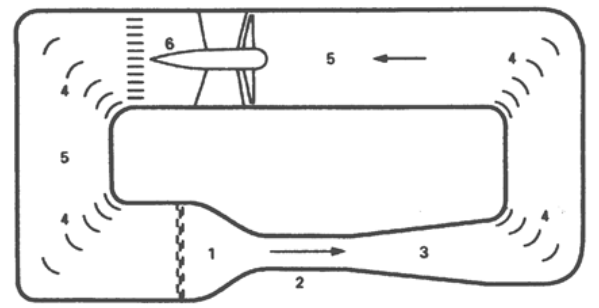
\includegraphics[width=60mm]{tunel_cerrado.png}}
    \subfigure[Túnel tipo abierto]{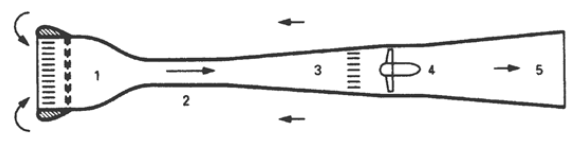
\includegraphics[width=80mm]{tunel_abierto.png}}
    \caption{Clasificación túneles} \label{fig:abierto}
    \end{figure}


\subsection{Historia del Túnel UNPSJB}

\begin{wrapfigure}{r}{0.5\textwidth} 
	\begin{center}
		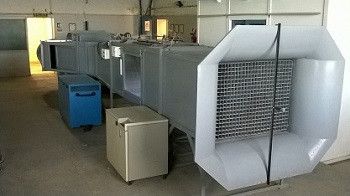
\includegraphics[scale=0.45]{tunel_unpsjb.JPG}
		\captionof{figure}{Tunel UNPSJB}
		\label{fig:tunelUni}
	\end{center}
	\vspace{-20pt}
	\end{wrapfigure}


\footnote{http://www.ing.unp.edu.ar/mecanica/Paginas/Tunel.htm} 
	El túnel aerodinámico del Laboratorio de Mecánica de Fluidos (LMF) de la Facultad de Ingeniería de la Universidad Nacional de la Patagonia San Juan Bosco (UNPSJB) es un circuito abierto (tipo Eiffel) con cámara de ensayos cerrada. Puede clasificarse como un túnel “pequeño de baja velocidad”, con una longitud total de 11m, una velocidad máxima de 18 m/s y una cámara de ensayos con un área de 0,8m2.
	\\
	La entrada del túnel cuenta con canalizadores, comúnmente denominados "panal de abejas", que favorecen la formación de un flujo uniforme y homogéneo propiciando mejores resultados en los experimentos.
	\\
	La cámara de ensayos es vidriada para poder observar con claridad el flujo y está incorporada en un módulo extraíble del túnel, lo cual permite fácil acceso para el armado de los distintos objetos a ensayar.
	\\
	La variación de la velocidad del aire dentro de la cámara se consigue por dos vías: modificando la velocidad del motor para lograr una aproximación, y mediante la apertura de compuertas ubicadas entre el rodete y la zona de ensayo, para el ajuste fino. La toma aire desde el exterior a través de las compuertas actúa como by-pass, modificando el flujo principal del túnel y controlando su velocidad.
	\\
	Los distintos ensayos que se realizan en el túnel son:
	\\
	- Determinación de coeficientes de resistencia y sustentación de distintos cuerpos y perfiles aerodinámicos. \\
	- Determinación de distribución de presiones a través de diferentes objetos como perfiles aerodinámicos, edificios, puentes, automóviles, etc. \\
	- Visualización con humo del flujo a través de distintos obstáculos. \\
	- Estudio del comportamiento dinámico de generadores eólicos. \\
	- Calibración de anemómetros. 
	\\
		\subsubsection{Motor y Variador de velocidad}
		\begin{tcolorbox}[colback=blue!5!white,colframe=blue!75!black,title=Variador de velocidad]
			Es utilizado para controlar la velocidad de giro de un motor. Para regular lasrevoluciones, se debe tener en cuenta las características del motor, ya que estetiene  una  curva  propia  de  funcionamiento.  Un  variador  es  capaz  de  generarelementos  control  de  aceleración,  frenado,  seguridad,  control  del  torque  yoperaciones que mejoran la eficiencia energética..\end{tcolorbox}	

	\footnote{\url{http://www.ing.unp.edu.ar/mecanica/Archivos/Fluid/LMF/Informe_Proyecto_-_Túnel_de_Viento.pdf}}
El motor que se utiliza en el túnel corresponde a uno donado por la empresa YPF, de pocos datos. Mientras que el variador de velocidad es de la marca Long Shenq.

\paragraph*{Especificaciones}
	\begin{minipage}[t]{.7\textwidth}
		\begin{itemize}
			\item LS650-4045
			\item Potencia: 45kW / 60HP
			\item Salida trifásica
		\end{itemize}
	\end{minipage}	
	\begin{minipage}[t]{.3\textwidth}
		\centering\raisebox{\dimexpr \topskip-\height}{%
		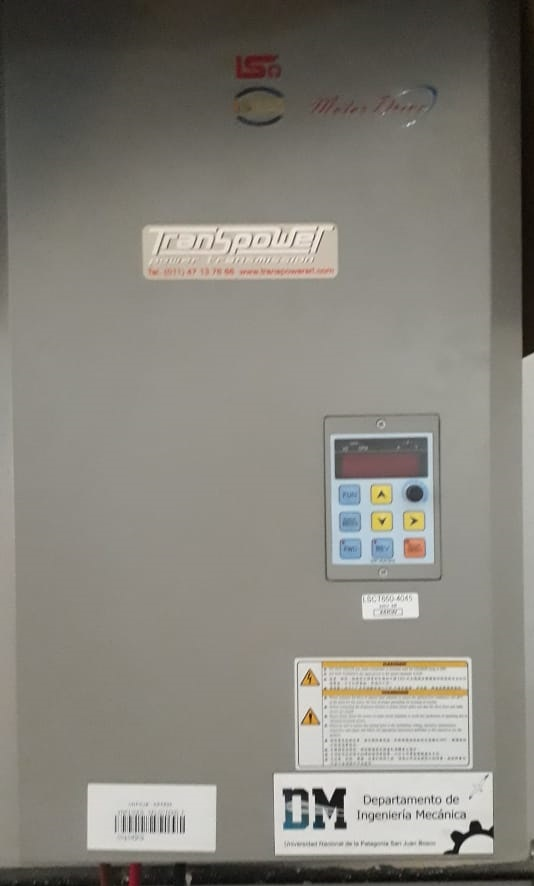
\includegraphics[scale=0.35]{LS650.jpg}}
		\captionof{figure}{LS650}
		\label{fig:LS650}
	\end{minipage}

		
		\newpage